\documentclass[aspectratio=169]{beamer}
\usetheme[sectionpage=progressbar, subsectionpage=progressbar, progressbar=frametitle, numbering=fraction, block=fill]{metropolis}

% Math packages
\usepackage{amsmath}
\usepackage{amssymb}
\usepackage{amsthm}
\usepackage{mathtools}

\usepackage{appendixnumberbeamer}

\usepackage{tikz}
\usetikzlibrary{automata, positioning, arrows, calc, fit, shapes.misc}

% Colors
\usepackage{xcolor} %already loaded by tikz, but here for completeness
% RWTH colors
% blue violet purple carmine red magenta orange yellow grass cyan gold silver
\definecolor{rwth-blue}{cmyk}{1,.5,0,0}\colorlet{rwth-lblue}{rwth-blue!50}\colorlet{rwth-llblue}{rwth-blue!25}
\definecolor{rwth-violet}{cmyk}{.6,.6,0,0}\colorlet{rwth-lviolet}{rwth-violet!50}\colorlet{rwth-llviolet}{rwth-violet!25}
\definecolor{rwth-purple}{cmyk}{.7,1,.35,.15}\colorlet{rwth-lpurple}{rwth-purple!50}\colorlet{rwth-llpurple}{rwth-purple!25}
\definecolor{rwth-carmine}{cmyk}{.25,1,.7,.2}\colorlet{rwth-lcarmine}{rwth-carmine!50}\colorlet{rwth-llcarmine}{rwth-carmine!25}
\definecolor{rwth-red}{cmyk}{.15,1,1,0}\colorlet{rwth-lred}{rwth-red!50}\colorlet{rwth-llred}{rwth-red!25}
\definecolor{rwth-magenta}{cmyk}{0,1,.25,0}\colorlet{rwth-lmagenta}{rwth-magenta!50}\colorlet{rwth-llmagenta}{rwth-magenta!25}
\definecolor{rwth-orange}{cmyk}{0,.4,1,0}\colorlet{rwth-lorange}{rwth-orange!50}\colorlet{rwth-llorange}{rwth-orange!25}
\definecolor{rwth-yellow}{cmyk}{0,0,1,0}\colorlet{rwth-lyellow}{rwth-yellow!50}\colorlet{rwth-llyellow}{rwth-yellow!25}
\definecolor{rwth-grass}{cmyk}{.35,0,1,0}\colorlet{rwth-lgrass}{rwth-grass!50}\colorlet{rwth-llgrass}{rwth-grass!25}
\definecolor{rwth-green}{cmyk}{.7,0,1,0}\colorlet{rwth-lgreen}{rwth-green!50}\colorlet{rwth-llgreen}{rwth-green!25}
\definecolor{rwth-cyan}{cmyk}{1,0,.4,0}\colorlet{rwth-lcyan}{rwth-cyan!50}\colorlet{rwth-llcyan}{rwth-cyan!25}
\definecolor{rwth-teal}{cmyk}{1,.3,.5,.3}\colorlet{rwth-lteal}{rwth-teal!50}\colorlet{rwth-llteal}{rwth-teal!25}
\definecolor{rwth-gold}{cmyk}{.35,.46,.7,.35}
\definecolor{rwth-silver}{cmyk}{.39,.31,.32,.14}


\usepackage{multicol}

\usepackage{todonotes}

\usepackage{subcaption}

% Custom commands
\newcommand{\GFC}{\mathsf{GF}(\mathsf{C})}
\newcommand{\free}[1]{\operatorname{free}(#1)}
\newcommand{\gd}[1]{\operatorname{gd}(#1)}
\newcommand{\RCR}{\operatorname{RCR}}
\newcommand{\CR}{\operatorname{CR}}
\newcommand{\disjunctiveGFC}{\operatorname{disjunctive-\GFC}}
\newcommand{\set}{\operatorname{set}}
\newcommand{\ipo}{i+1\operatorname{mod}}
\newcommand{\Hom}{\operatorname{Hom}}
\newcommand{\C}[1]{\mathsf{C}_{#1}}
\newcommand{\atp}{\operatorname{atp}}
\newcommand{\stp}{\operatorname{stp}}

\newcommand{\term}[1]{\operatorname{\mathit{#1}}}

\renewcommand{\theta}{\vartheta}
\renewcommand{\rho}{\varrho}

\renewcommand{\phi}{\varphi}
\renewcommand{\epsilon}{\varepsilon}

\def\multiset#1{\ensuremath{\left\{\kern-.35em\left\{#1\right\}\kern-.35em\right\}}}
\newcommand{\leftmultiset}{\ensuremath{\{\kern-.35em\{}}
\newcommand{\rightmultiset}{\ensuremath{\}\kern-.35em\}}}


\title{Relational Colour Refinement for Non-Relational Signatures}
\date{September 5, 2025}
\author{Theodor Jurij Teslia}
\institute{RWTH Aachen University}



\begin{document}
	
	\maketitle
	
	\begin{frame}{Introduction}
		\begin{itemize}
			\item Colour Refinement is an important and interesting algorithm
			\item Applied in modern isomorphism solvers
			\item Can be characterised logically and combinatorially
			\item Extension to more than graphs seems desirable
			\item Scheidt and Schweikardt \textcolor{red}{bibliography} introduced Relational Colour Refinement
			\item Conceptually similar to classical Colour Refinement
			\item Also has a logical and a combinatorial characterisation
		\end{itemize}
	\end{frame}
	
	\begin{frame}{Contents of this presentation}
		\setbeamertemplate{section in toc}[sections numbered]
		\tableofcontents[hideallsubsections]
	\end{frame}
	
	\section{Classical Colour Refinement}
	
	\begin{frame}{Colour Refinement}
		\begin{itemize}
			\item Also called \emph{CR} or \emph{$1$-dimensional Weisfeiler-Leman} algorithm
			\item Iterative graph algorithm
			\item Constructs colour for every vertex, based on colours of neighbours
		\end{itemize}
		
		\begin{definition}[Colour Refinement]
			For graph $G=(V,E)$, for every $v\in V$ and $i\in \mathbb N$:
			\begin{itemize}
				\item Initial colour: $C_0(v)\coloneqq 0$
				\item Next rounds:$$C_{i+1}(v)\coloneqq(C_i(v),\multiset{C_i(u) : \{v,u\}\in E})$$
			\end{itemize}
		\end{definition}
	\end{frame}
	
	\begin{frame}{Example for CR}
		\begin{columns}
			\begin{column}{0.25\textwidth}
				\centering
				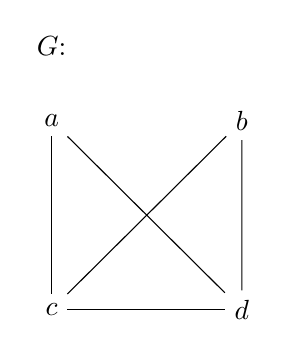
\begin{tikzpicture}[node distance=2cm]
					\node (a) {$a$};
					\node[right=of a] (b) {$b$};
					\node[below=of a] (c) {$c$};
					\node[right=of c] (d) {$d$};
					\node[above=of a, yshift=-1.5cm] (name) {$G$:};
					
					\draw
					(a) edge[-] (c)
						edge[-] (d)
					(b) edge[-] (c)
						edge[-] (d)
					(c) edge[-] (d);
				\end{tikzpicture}
			\end{column}
			\begin{column}{0.75\textwidth}
				\begin{itemize}
					\item $C_0(a)=C_0(b)=C_0(c)=C_0(d)=0$
					\item[]
					\item $C_1(a)=C_1(b)=(0,\multiset{0, 0})$
					\item $C_1(c)=C_1(d)=(0,\multiset{0, 0, 0})$
				\end{itemize}
			\end{column}
		\end{columns}
	\end{frame}
	
	\begin{frame}{Distinguished graphs}
		\begin{itemize}
			\item CR distinguishes two graphs $G$ and $H$, if
			\item there exists $C_i(v)$ in colouring of $G$ or $H$, such that the number of vertices with colour $C_i(v)$ is different in $G$ than in $H$
		\end{itemize}
		\pause
		\begin{columns}
			\begin{column}{0.25\textwidth}
				\centering
				\begin{tikzpicture}[node distance=2cm]
					\node (a) {$a'$};
					\node[right=of a] (b) {$b'$};
					\node[below=of a] (c) {$c'$};
					\node[right=of c] (d) {$d'$};
					\node[above=of a, yshift=-1.5cm] (name) {$H$:};
					
					\draw
					(a) edge[-] (c)
					edge[-] (d)
					(b) edge[-] (d)
					(c) edge[-] (d);
				\end{tikzpicture}
			\end{column}
			\begin{column}{0.75\textwidth}
				\begin{itemize}
					\item Colours in first round equal
					\item $C_1(b')=(0, \multiset{0})$ does not appear in $G$
					\item[]
					\item[$\Rightarrow$] Colour Refinement distinguishes $G$ and $H$
				\end{itemize}
			\end{column}
		\end{columns}
	\end{frame}
	
	\begin{frame}{Characterisations of CR}
		\begin{itemize}
			\item There are equivalent characterisations for CR
			\item Due to \textcolor{red}{bibliography}:\break
			CR distinguishes $G$ and $H$ if, and only if, there exists $\phi\in \C{2}$, such that $G\models \phi$ and $H\not\models \phi$
			\item Due to \textcolor{red}{bibliography}:\break
			CR distinguishes $G$ and $H$ if, and only if, there exists tree $T$, such that $\hom(T,G)\neq\hom(T,H)$
		\end{itemize}
	\end{frame}
	
	\begin{frame}{Application of Characterisations to Example}
			\begin{columns}
			\begin{column}{0.25\textwidth}
				\centering
				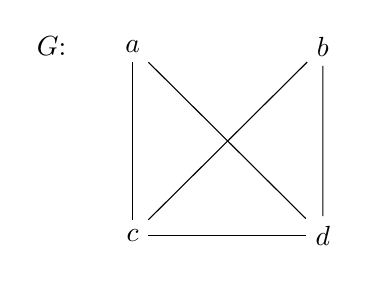
\begin{tikzpicture}[node distance=2cm]
					\node (a) {$a$};
					\node[right=of a] (b) {$b$};
					\node[below=of a] (c) {$c$};
					\node[right=of c] (d) {$d$};
					\node[left=of a, xshift=1.5cm] (name) {$G$:};
					
					\draw
					(a) edge[-] (c)
					edge[-] (d)
					(b) edge[-] (c)
					edge[-] (d)
					(c) edge[-] (d);
				\end{tikzpicture}
				
			\end{column}
			\begin{column}{0.75\textwidth}
				\begin{itemize}
					\item Used existence of colour $(0,\multiset{0})$ in colouring of $H$ to distinguish $G$ and $H$
					\item From colour it follows that vertex with degree $1$ exists
					\item $\exists^{\geq 1} x \operatorname{.} \exists^{=1} y \operatorname{.} E(x,y)$ distinguishes $G$ and $H$
				\end{itemize}
			\end{column}
		\end{columns}
		\begin{columns}
			\begin{column}{0.25\textwidth}
				\centering
				\begin{tikzpicture}[node distance=2cm]
					\node (a) {$a'$};
					\node[right=of a] (b) {$b'$};
					\node[below=of a] (c) {$c'$};
					\node[right=of c] (d) {$d'$};
					\node[left=of a, xshift=1.5cm] (name) {$H$:};
					
					\draw
					(a) edge[-] (c)
					edge[-] (d)
					(b) edge[-] (d)
					(c) edge[-] (d);
				\end{tikzpicture}
			\end{column}
			\begin{column}{0.75\textwidth}
				\onslide<2>{
					\begin{itemize}
						\item There are $5$ edges in $G$ but only $4$ in $H$
						\item Tree $T\coloneqq(\{v, u\}, \{\{v,u\}\})$ has $10$ homomorphisms to $G$ and $8$ to $H$
					\end{itemize}
				}
			\end{column}
		\end{columns}
	\end{frame}
	
	\section{Relational Colour Refinement}
	
	\begin{frame}{Relational Colour Refinement}
		\begin{itemize}
			\item Called \emph{RCR} for short
			\item Applies variant of classical Colour Refinement on tuples of structure
			\item Uses atomic type as part of initial colouring
			\item Uses pairs of indices as edges to mark shared elements of tuples
			\item Formally:
			$$\operatorname{atp}(\mathbf a) = \{ R \in \sigma : \mathbf a \in R\}$$
			and
			$$\operatorname{stp}(\mathbf a, \mathbf b)=\{(i,j)\in [n]\times[m] : a_i = b_j\}$$
		\end{itemize}
	\end{frame}
	
	\begin{frame}{The Algorithm}
		\begin{itemize}
			\item For relational structure $\mathfrak A$ and all tuples $\mathbf a\in \mathbf A$:
			\item Initial colour: $\varrho_0(\mathbf a)=(\operatorname{atp}(\mathbf a), \operatorname{stp}(\mathbf a, \mathbf a))$
			\item For the next rounds: $\varrho_{i+1}(\mathbf a)=(\varrho_i(\mathbf a), \multiset{(\operatorname{stp}(\mathbf a,\mathbf b), \varrho_i(\mathbf b)) : \set(\mathbf a)\cap\set(\mathbf b)\neq\emptyset})$
		\end{itemize}
	\end{frame}
	
	\begin{frame}{An Example for RCR}
		\begin{columns}
			\begin{column}{0.25\textwidth}
				\centering
				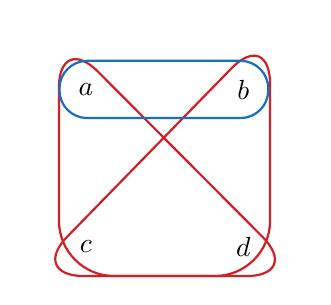
\begin{tikzpicture}
					\node[] at (0,0) (a) {$a$};
					\node[] at (2, 0) (b) {$b$};
					\node[] at (0, -2) (c) {$c$};
					\node[] at (2, -2) (d) {$d$};
					
					\node[fit=(a) (c) (d)] (acd) {};
					\draw[rounded corners=20pt, thick, rwth-red] ($(acd.north west)+(0,0.4)$) -- (acd.south west) -- ($(acd.south east)+(0.4,0)$) -- cycle;
					
					\node[fit=(b) (c) (d)] (bcd) {};
					\draw[rounded corners=20pt, thick, rwth-red] ($(bcd.north east)+(0,0.4)$) -- (bcd.south east) -- ($(bcd.south west)+(-0.4, 0)$) -- cycle;
					
					\node[draw, rounded corners=10pt, thick, rwth-blue, fit=(a) (b)] {};
				\end{tikzpicture}
			\end{column}
			\begin{column}{0.75\textwidth}
				\begin{itemize}
					\item Structure $\mathfrak A=(A,R^{\mathfrak A},T^{\mathfrak A})$
					\item $A=\{a,b,c,d\}$, $R^{\mathfrak A}=\{(a,b)\}$, $T^{\mathfrak A}=\{(a,c,d),(b,c,d)\}$
				\end{itemize}
			\end{column}
		\end{columns}
		\begin{itemize}
			\item $\rho_0((a,b))=(\{R\},\{(1,1),(2,2)\})$ and $\rho_0((a,c,d))=\rho_0((b,c,d))=(\{T\}, \{(1,1),(2,2),(3,3)\})$
			\item $\rho_1((a,c,d))=(\rho_0((a,c,d)), \multiset{(\{(1,1)\}, \rho_0((a,b))), \dots})$
			and 
			$\rho_1((b,c,d))=(\rho_0((b,c,d)), \multiset{(\{(1,2)\}, \rho_0((a,b))), \dots})$
		\end{itemize}
	\end{frame}
	
	\begin{frame}{Distinguishing Relational Structures with RCR}
		\begin{itemize}
			\item RCR distinguishes, if some colour appears differently often in the structures
		\end{itemize}
		\begin{columns}
			\begin{column}{0.5\textwidth}
				\centering
				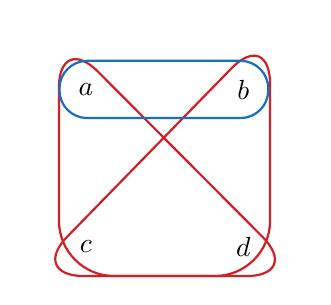
\begin{tikzpicture}
					\node[] at (0,0) (a) {$a$};
					\node[] at (2, 0) (b) {$b$};
					\node[] at (0, -2) (c) {$c$};
					\node[] at (2, -2) (d) {$d$};
					
					\node[fit=(a) (c) (d)] (acd) {};
					\draw[rounded corners=20pt, thick, rwth-red] ($(acd.north west)+(0,0.4)$) -- (acd.south west) -- ($(acd.south east)+(0.4,0)$) -- cycle;
					
					\node[fit=(b) (c) (d)] (bcd) {};
					\draw[rounded corners=20pt, thick, rwth-red] ($(bcd.north east)+(0,0.4)$) -- (bcd.south east) -- ($(bcd.south west)+(-0.4, 0)$) -- cycle;
					
					\node[draw, rounded corners=10pt, thick, rwth-blue, fit=(a) (b)] {};
				\end{tikzpicture}
			\end{column}
			\begin{column}{0.5\textwidth}
				\centering
				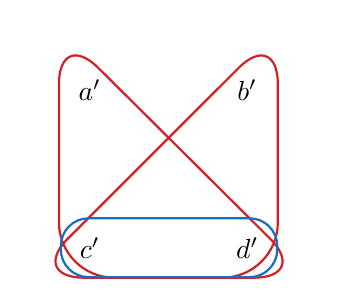
\begin{tikzpicture}
					\node[] at (0,0) (a) {$a'$};
					\node[] at (2, 0) (b) {$b'$};
					\node[] at (0, -2) (c) {$c'$};
					\node[] at (2, -2) (d) {$d'$};
					
					\node[fit=(a) (c) (d)] (acd) {};
					\draw[rounded corners=20pt, thick, rwth-red] ($(acd.north west)+(0,0.4)$) -- (acd.south west) -- ($(acd.south east)+(0.4,0)$) -- cycle;
					
					\node[fit=(b) (c) (d)] (bcd) {};
					\draw[rounded corners=20pt, thick, rwth-red] ($(bcd.north east)+(0,0.4)$) -- (bcd.south east) -- ($(bcd.south west)+(-0.4, 0)$) -- cycle;
					
					\node[draw, rounded corners=10pt, thick, rwth-blue, fit=(c) (d)] {};
				\end{tikzpicture}
			\end{column}
		\end{columns}
		\begin{itemize}
			\item $\rho_1((a,c,d))$ appears in colouring of left structure but not in right
		\end{itemize}
	\end{frame}
	
	\subsection{Logical Characterisation of RCR}
	
	\begin{frame}{Guarded Fragment of Counting Logic}
		\begin{itemize}
			\item $\C{2}$ characterises CR on graphs
			\item Guarded fragment of counting logic $\GFC$ characterises RCR
		\end{itemize}
		
		\begin{block}{Guarded Fragment of Counting Logic}
			\begin{itemize}
				\item Everything except for quantifiers defined as in classical counting logic
				\item For atomic formula $\Delta\in\GFC$ and formula $\phi\in\GFC$, we call $\Delta$ a guard for $\phi$, if $\free{\Delta}\supseteq \free{\phi}$
				\item Quantifiers appear only in form $\exists^{\geq i} \mathbf v \operatorname{.} (\Delta \land \phi)$, where $\Delta$ is guard for $\phi$ and $\set(\mathbf v) \subseteq \free{\Delta}$
			\end{itemize}
		\end{block}
		\begin{itemize}
			\item Examples: 
			\begin{itemize}
				\item $\exists^{\geq 2} (x,y) \operatorname{.}(E(x,y)\land T(y))\in \GFC$
				\item $\exists^{\geq 3} (x,y,z) \operatorname{.} (E(x,y) \land E(y,z) \land E(z,x))\notin \GFC$
			\end{itemize}
		\end{itemize}
	\end{frame}
	
	\begin{frame}{Characterising RCR Using Logic}
		\begin{block}{Theorem B from \textcolor{red}{bibliography}}
			Let $\mathfrak A$ and $\mathfrak B$ be two relational structures.
			Then the two following statements are equivalent.
			\begin{enumerate}
				\item RCR distinguishes $\mathfrak A$ and $\mathfrak B$
				\item There exists a sentence in $\GFC$ that is satisfied by $\mathfrak A$, but not by $\mathfrak B$
			\end{enumerate}
		\end{block}
	\end{frame}
	
	\begin{frame}{Example for Logical Characterisation of RCR}
		\begin{columns}
			\begin{column}{0.5\textwidth}
				\centering
				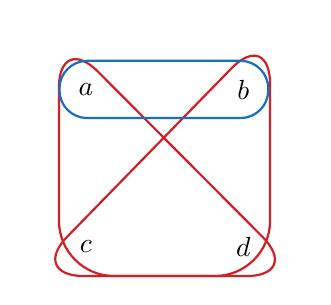
\begin{tikzpicture}
					\node[] at (0,0) (a) {$a$};
					\node[] at (2, 0) (b) {$b$};
					\node[] at (0, -2) (c) {$c$};
					\node[] at (2, -2) (d) {$d$};
					
					\node[fit=(a) (c) (d)] (acd) {};
					\draw[rounded corners=20pt, thick, rwth-red] ($(acd.north west)+(0,0.4)$) -- (acd.south west) -- ($(acd.south east)+(0.4,0)$) -- cycle;
					
					\node[fit=(b) (c) (d)] (bcd) {};
					\draw[rounded corners=20pt, thick, rwth-red] ($(bcd.north east)+(0,0.4)$) -- (bcd.south east) -- ($(bcd.south west)+(-0.4, 0)$) -- cycle;
					
					\node[draw, rounded corners=10pt, thick, rwth-blue, fit=(a) (b)] {};
				\end{tikzpicture}
			\end{column}
			\begin{column}{0.5\textwidth}
				\centering
				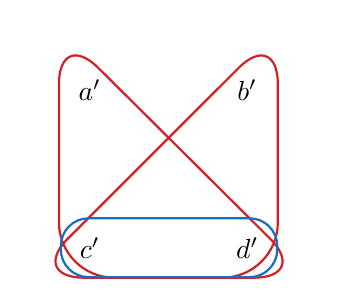
\begin{tikzpicture}
					\node[] at (0,0) (a) {$a'$};
					\node[] at (2, 0) (b) {$b'$};
					\node[] at (0, -2) (c) {$c'$};
					\node[] at (2, -2) (d) {$d'$};
					
					\node[fit=(a) (c) (d)] (acd) {};
					\draw[rounded corners=20pt, thick, rwth-red] ($(acd.north west)+(0,0.4)$) -- (acd.south west) -- ($(acd.south east)+(0.4,0)$) -- cycle;
					
					\node[fit=(b) (c) (d)] (bcd) {};
					\draw[rounded corners=20pt, thick, rwth-red] ($(bcd.north east)+(0,0.4)$) -- (bcd.south east) -- ($(bcd.south west)+(-0.4, 0)$) -- cycle;
					
					\node[draw, rounded corners=10pt, thick, rwth-blue, fit=(c) (d)] {};
				\end{tikzpicture}
			\end{column}
		\end{columns}
		\begin{itemize}
			\item We have seen RCR distinguishes the structures
			\item Formula $\exists^{\geq 1}(x,y,z).\left(T(x,y,z)\land \exists^{\geq 1} (y).\left( R(x,y)\right)\right)$ satisfied by left and not by right structure
		\end{itemize}
	\end{frame}
	
	\subsection{Combinatorial Characterisation of RCR}
	
	\begin{frame}{Acyclic Structures}
		\begin{itemize}
			\item Counting homomorphisms from trees characterises CR on graphs
			\item Abstraction from trees to relational structures is needed: $\alpha$-acyclic structures (in the following only acyclic structures)
		\end{itemize}
		\begin{block}{Acyclic Structures}
			\begin{itemize}
				\item Let $\mathfrak C$ be relational structure
				\item Join tree $J$ for $\mathfrak C$ is tree with $V(J)=\mathbf C$ and fulfils join-tree-property:
				\begin{itemize}
					\item For every $e\in C$, the set $\{\mathbf x \in V(J) : e\in \mathbf \set(x)\}$ induces a connected subtree
				\end{itemize}
				\item We call $\mathfrak C$ acyclic, if it has a join tree
			\end{itemize}
		\end{block}
	\end{frame}
	
	% Animations?
	\begin{frame}{Examples for Acyclic Structures}
		\begin{columns}
			\begin{column}{0.4\textwidth}
				\centering
				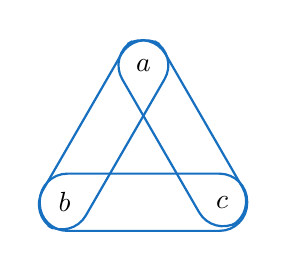
\begin{tikzpicture}
					\node[] at (1,1.73) (a) {$a$};
					\node[] at (0, 0) (b) {$b$};
					\node[] at (2, 0) (c) {$c$};
					
					\node[] at (0, 2.1) (left) {};
					\node[draw, rounded corners=10pt, thick, rwth-blue, fit=(b) (left), rotate around={-30:(b)}] {};
					
					\node[] at (2, 2.1) (right) {};
					\node[draw, rounded corners=10pt, thick, rwth-blue, fit=(c) (right), rotate around={30:(c)}] {};
					
					\node[draw, rounded corners=10pt, thick, rwth-blue, fit=(b) (c)] {};
				\end{tikzpicture}
			\end{column}
			\begin{column}{0.2\textwidth}
				\centering
				\hfill No:
			\end{column}
			\begin{column}{0.4\textwidth}
				\centering
				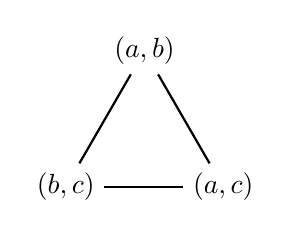
\begin{tikzpicture}
					\node[] at (1,1.73) (ab) {$(a,b)$};
					\node[] at (0,0) (bc) {$(b,c)$};
					\node[] at (2,0) (ac) {$(a,c)$};
					
					\draw
					(ab) edge[-, thick] (bc)
					(ab) edge[-, thick] (ac)
					(bc) edge[-, thick] (ac);
				\end{tikzpicture}
			\end{column}
		\end{columns}
		\pause
		\vspace{10pt}
		\begin{columns}
			\begin{column}{0.4\textwidth}
				\centering
				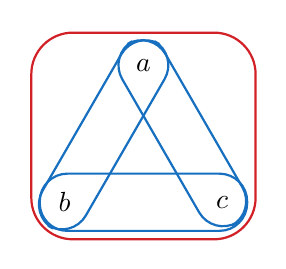
\begin{tikzpicture}
					\node[] at (1,1.73) (a) {$a$};
					\node[] at (0, 0) (b) {$b$};
					\node[] at (2, 0) (c) {$c$};
					
					\node[] at (0, 2.1) (left) {};
					\node[draw, rounded corners=10pt, thick, rwth-blue, fit=(b) (left), rotate around={-30:(b)}] {};
					
					\node[] at (2, 2.1) (right) {};
					\node[draw, rounded corners=10pt, thick, rwth-blue, fit=(c) (right), rotate around={30:(c)}] {};
					
					\node[draw, rounded corners=10pt, thick, rwth-blue, fit=(b) (c)] {};
					
					\node[fit=(a) (b) (c)] (abc) {};
					\draw[rounded corners=15pt, thick, rwth-red] ($(abc.north west)+(-0.1,0.1)$) -- ($(abc.south west)+(-0.1,-0.1)$) -- ($(abc.south east)+(0.1,-0.1)$) -- ($(abc.north east)+(0.1,0.1)$) -- cycle;
				\end{tikzpicture}
			\end{column}
			\begin{column}{0.2\textwidth}
				\centering
				\hfill Yes:
			\end{column}
			\begin{column}{0.4\textwidth}
				\centering
				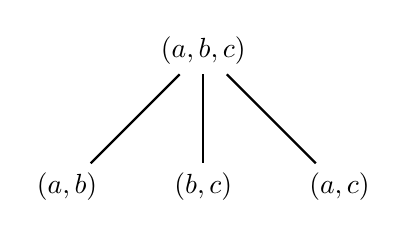
\begin{tikzpicture}
					\node[] at (0, 0) (abc) {$(a,b,c)$};
					\node[] at (-1.73,-1.73) (ab) {$(a,b)$};
					\node[] at (0,-1.73) (bc) {$(b,c)$};
					\node[] at (1.73,-1.73) (ac) {$(a,c)$};
					
					\draw
					(abc) edge[-, thick] (ab)
					(abc) edge[-, thick] (ac)
					(abc) edge[-, thick] (bc);
				\end{tikzpicture}
			\end{column}
		\end{columns}
	\end{frame}
	
	\begin{frame}{Characterising RCR Using Homomorphism Counting}
		\begin{block}{Theorem A from \textcolor{red}{bibliography}}
			Let $\mathfrak A$ and $\mathfrak B$ be relational structures.
			Then the two following statements are equivalent.
			\begin{enumerate}
				\item RCR distinguishes $\mathfrak A$ and $\mathfrak B$
				\item There exists an acyclic relational structure $\mathfrak C$, such that it has a different number of homomorphisms to $\mathfrak A$ than to $\mathfrak B$
			\end{enumerate}
		\end{block}
	\end{frame}
	
	\begin{frame}{Example for Combinatorial Characterisation of RCR}
		\begin{columns}
			\begin{column}{0.33\textwidth}
				\centering
				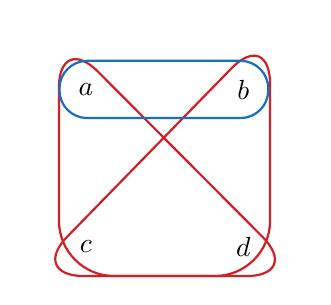
\begin{tikzpicture}
					\node[] at (0,0) (a) {$a$};
					\node[] at (2, 0) (b) {$b$};
					\node[] at (0, -2) (c) {$c$};
					\node[] at (2, -2) (d) {$d$};
					
					\node[fit=(a) (c) (d)] (acd) {};
					\draw[rounded corners=20pt, thick, rwth-red] ($(acd.north west)+(0,0.4)$) -- (acd.south west) -- ($(acd.south east)+(0.4,0)$) -- cycle;
					
					\node[fit=(b) (c) (d)] (bcd) {};
					\draw[rounded corners=20pt, thick, rwth-red] ($(bcd.north east)+(0,0.4)$) -- (bcd.south east) -- ($(bcd.south west)+(-0.4, 0)$) -- cycle;
					
					\node[draw, rounded corners=10pt, thick, rwth-blue, fit=(a) (b)] {};
				\end{tikzpicture}
			\end{column}
			\begin{column}{0.33\textwidth}
				\centering
				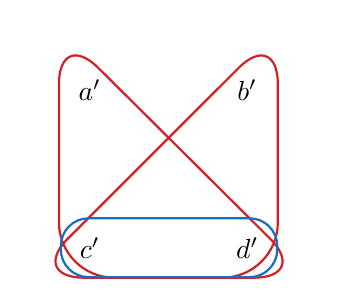
\begin{tikzpicture}
					\node[] at (0,0) (a) {$a'$};
					\node[] at (2, 0) (b) {$b'$};
					\node[] at (0, -2) (c) {$c'$};
					\node[] at (2, -2) (d) {$d'$};
					
					\node[fit=(a) (c) (d)] (acd) {};
					\draw[rounded corners=20pt, thick, rwth-red] ($(acd.north west)+(0,0.4)$) -- (acd.south west) -- ($(acd.south east)+(0.4,0)$) -- cycle;
					
					\node[fit=(b) (c) (d)] (bcd) {};
					\draw[rounded corners=20pt, thick, rwth-red] ($(bcd.north east)+(0,0.4)$) -- (bcd.south east) -- ($(bcd.south west)+(-0.4, 0)$) -- cycle;
					
					\node[draw, rounded corners=10pt, thick, rwth-blue, fit=(c) (d)] {};
				\end{tikzpicture}
			\end{column}
			\begin{column}{0.33\textwidth}
				\vspace{13pt}
				\centering
				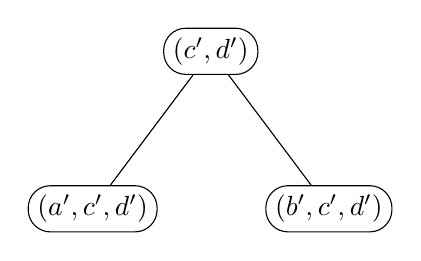
\begin{tikzpicture}
					\node[draw, rounded corners=8pt] at (0, 0) (cd) {$(c',d')$};
					\node[draw, rounded corners=8pt] at (-1.5, -2) (acd) {$(a',c',d')$};
					\node[draw, rounded corners=8pt] at (1.5, -2) (bcd) {$(b',c',d')$};
					
					\draw
					(cd) edge[-] (acd)
					(cd) edge[-] (bcd);
				\end{tikzpicture}
			\end{column}
		\end{columns}
		\vspace{10pt}
		\begin{itemize}
			\item Right tree is join tree for middle structure, therefore middle structure is acyclic
			\item Identity is homomorphism, so middle structure has at least one homomorphism to itself
			\item Middle structure has no homomorphisms to left structure
		\end{itemize}
	\end{frame}
	
	\section{Relational Colour Refinement for Structures With Functions}
	
	\begin{frame}{Relational Colour Refinement for Structures With Functions}
		\begin{itemize}
			\item Many interesting structures use functions
			\item Colour Refinement algorithm for such structures seems desirable
			\item Will use the results of Scheidt and Schweikardt \textcolor{red}{bibliography} and investigate how robust they are
			\item Following structure:
			\begin{enumerate}
				\item Presentation of two approaches for Colour Refinement for non-relational signatures
				\item Logical characterisation of both approaches
				\item Discussion on combinatorial characterisation
			\end{enumerate}
		\end{itemize}
	\end{frame}
	
	\begin{frame}{Naive RCR}
		\begin{itemize}
			\item Goal: Encode non-relational structures and signatures as relational ones
			\item Functions can directly be interpreted as relations:
			$$f(\mathbf x)=y \Longleftrightarrow (\mathbf xy)\in R_f$$
			\item For non-relational signature $\sigma$ define relational signature $\sigma'$:
			\begin{itemize}
				\item Relation symbol $R\in\sigma$ of arity $n$ $\rightarrow$ introduce $R\in\sigma'$ of arity $n$
				\item Function symbol $f\in\sigma$ of arity $n$ $\rightarrow$ introduce $R_f\in\sigma'$ of arity $n+1$
			\end{itemize}
			\item Encode $\sigma$-structure $\mathfrak A$ as $\sigma'$-structure $\mathfrak A'$:
			\begin{itemize}
				\item For relation symbol $R\in\sigma$: $R^{\mathfrak A'}\coloneqq R^{\mathfrak A}$
				\item For function symbol $f\in \sigma$: $R_f^{\mathfrak A'}\coloneqq \{(\mathbf xy) : f^{\mathfrak A}(\mathbf x)=y\}$
			\end{itemize}
			\item We say naive RCR distinguishes $\mathfrak A$ and $\mathfrak B$, if RCR distinguishes the encodings
		\end{itemize}
	\end{frame}
	
	\begin{frame}{Idea of the Transitive Expansion}
		\begin{itemize}
			\item Approach is only defined for unary function symbols
			\item Encoding emulates the nesting of function applications
			\item Encode function $f$ as family of relations $R_{f^1},R_{f^2},\dots$, where $(x,y)\in R_{f^i}$ if $\underbrace{f(f(\dots f(}_{i\text{ times}}x)))=y$
			\item In the following: $f^i(x)$ written for $\underbrace{f(f(\dots f(}_{i\text{ times}}x)))$
			\item For multiple functions, also encode alternations, for example $R_{\term {fg}}$ or $R_{g^2f^3}$
		\end{itemize}
	\end{frame}
	
	\begin{frame}{Transitive Expansion i}
		\begin{block}{Alternations of Function Applications}
			\begin{itemize}
				\item Let $\sigma$ be signature with unary function symbols
				\item Define set of all allowed function application alternations $\operatorname{Alters}^k_n$ as $\operatorname{Alters}^0_n(\sigma)=\{\operatorname{id}\}$ and 
				\begin{align*}
					\operatorname{Alters}^k_{n}(\sigma)\coloneqq \operatorname{Alters}^{k-1}_{n}(\sigma)\cup\{f_1^{m_1}\dots f_k^{m_k} : & f_1,\dots, f_k\in \sigma_{\operatorname{Func}} \\ 
					& \land \forall i\in[k]\operatorname{.} m_i\in[n] \\ 
					& \land \forall i\in[k-1] \operatorname{.} f_{i} \neq f_{i+1}\}.
				\end{align*}
			\end{itemize}
		\end{block}
		\begin{itemize}
			\item Example: 
			\begin{itemize}
				\item $\sigma=\{f/1,g/1\}$
				\item $\operatorname{Alters}^2_2(\sigma)=\underbrace{\{\operatorname{id}\}}_{k=0} \cup \underbrace{\{f,f^2,g,g^2\}}_{k=1} \cup \underbrace{\{fg, fg^2, f^2g, f^2g^2, gf, \dots\}}_{k=2}$
			\end{itemize}
		\end{itemize}
	\end{frame}
	
	\begin{frame}{Transitive Expansion ii}
		\begin{block}{Transitive Expansion}
			\begin{itemize}
				\item For alternation depth $k$ and $\sigma$-structure $\mathfrak A$ with $\vert \mathfrak A\vert = n$ define transitive expansion $\widetilde{\mathfrak A}$ as a $\widetilde{\sigma}$-structure
				\item For $\alpha,\beta,\alpha_1,\dots,\alpha_\ell\in \operatorname{Alters}^k_n(\sigma)$ and relation symbol $R\in\sigma$ of arity $\ell$, insert relation symbol $\operatorname{Eq}_{\alpha,\beta}$ of arity $2$ and relation symbol $R_{\alpha_1,\dots,\alpha_\ell}$ of arity $\ell$ into $\widetilde{\sigma}$
				\item Define $\operatorname{Eq}_{\alpha,\beta}^{\widetilde{\mathfrak A}}\coloneqq \{(x,y) : \alpha^{\mathfrak A}(x)=\beta^{\mathfrak A}(y)\}$ and $R_{\alpha_1,\dots,\alpha_\ell}^{\widetilde{\mathfrak A}}\coloneqq \{(x_1,\dots,x_\ell) : (\alpha_1^{\mathfrak A}(x_1),\dots,\alpha_\ell^{\mathfrak A}(x_\ell))\in R^{\mathfrak A}\}$
			\end{itemize}
		\end{block}
		\begin{itemize}
			\item For $k\in\mathbb N$ we say that RCR$_k$ distinguishes structures $\mathfrak A$ and $\mathfrak B$, if RCR distinguishes the transitive expansions with alternation depth $k$
		\end{itemize}
	\end{frame}
	
	\begin{frame}{Example for the Transitive Expansion}
		\centering
		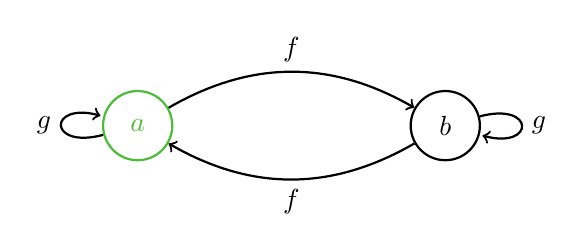
\begin{tikzpicture}[node distance=3cm]
			\node[state, rwth-green, thick] (a) {$a$};
			\node[state, right=of a, thick] (b) {$b$};
			%\node[left=of a, xshift=2cm] (label) {$\mathfrak A$:};
			\draw 
			(a) edge[->, thick, above, bend left] node{$f$} (b)
			(b) edge[->, thick, below, bend left] node{$f$} (a)
			(a) edge[->, thick, loop left] node{$g$} (a)
			(b) edge[->, thick, loop right] node{$g$} (b);
		\end{tikzpicture}
		\begin{itemize}
			\item Structure $\mathfrak A=(A,\textcolor{rwth-green}{R}^{\mathfrak A}, f^{\mathfrak A}, g^{\mathfrak A})$
			\item $k=1$ and $n=2$: $\operatorname{Alters}^1_2(\sigma)=\{\operatorname{id}, f,f^2,g,g^2\}$
			\item $\widetilde{\sigma}=\{R_{\operatorname{id}}, R_{f}, R_{f^2}, R_g, R_{g^2}, \operatorname{Eq}_{\operatorname{id},\operatorname{id}}, \operatorname{Eq}_{\operatorname{id},f}, \operatorname{Eq}_{\operatorname{id}, f^2}, \dots, \operatorname{Eq}_{g^2, g^2}\}$
			\item Examples:
			\begin{itemize}
				\item $R^{\widetilde{\mathfrak A}}_f=\{b\}$
				\item $\operatorname{Eq}_{f^2,\operatorname{id}}^{\widetilde{\mathfrak A}}=\{(a,a),(b,b)\}$
				\item $\operatorname{Eq}^{\widetilde{\mathfrak A}}_{g,f}=\{(a,b),(b,a)\}$
			\end{itemize}
		\end{itemize}
	\end{frame}
	
	\iffalse
	\begin{frame}{Naive Encoding versus Transitive Expansion}
		\begin{columns}
			\begin{column}{0.5\textwidth}
				\centering
				\scalebox{0.9}{
					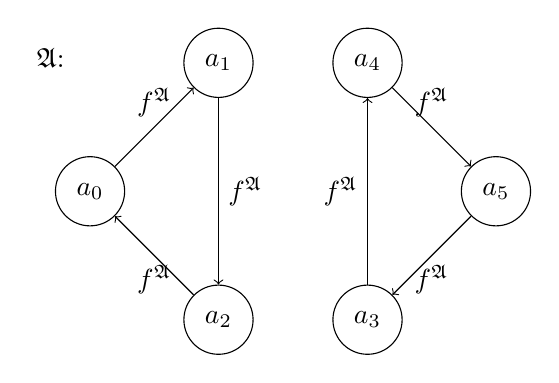
\begin{tikzpicture}
						\node[state] (a1) {$a_0$};
						\node[state, below right=of a1] (a3) {$a_2$};
						\node[state, above right=of a1] (a2) {$a_1$};
						\node[state, right =of a3] (a4) {$a_3$};
						\node[state, right =of a2] (a5) {$a_4$};
						\node[state, below right=of a5] (a6) {$a_5$};
						\node[above=of a1, xshift=-0.5cm] (label) {$\mathfrak A$:};
						\draw 
						(a1) edge[->, above] node{$f^{\mathfrak A}$} (a2)
						(a2) edge[->, right] node{$f^{\mathfrak A}$} (a3)
						(a3) edge[->, below] node{$f^{\mathfrak A}$} (a1)
						(a4) edge[->, left] node{$f^{\mathfrak A}$} (a5)
						(a5) edge[->, above] node{$f^{\mathfrak A}$} (a6)
						(a6) edge[->, below] node{$f^{\mathfrak A}$} (a4);
					\end{tikzpicture}
				}
			\end{column}
			\begin{column}{0.5\textwidth}
				\centering
				\scalebox{0.9}{
					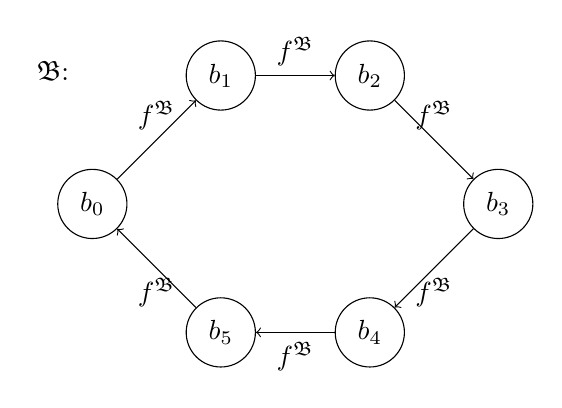
\begin{tikzpicture}
						\node[state] (b1) {$b_0$};
						\node[state, below right=of b1] (b6) {$b_5$};
						\node[state, above right=of b1] (b2) {$b_1$};
						\node[state, right =of b2] (b3) {$b_2$};
						\node[state, right =of b6] (b5) {$b_4$};
						\node[state, below right=of b3] (b4) {$b_3$};
						\node[above=of b1, xshift=-0.5cm] (label) {$\mathfrak B$:};
						\draw 
						(b1) edge[->, above] node{$f^{\mathfrak B}$} (b2)
						(b2) edge[->, above] node{$f^{\mathfrak B}$} (b3)
						(b3) edge[->, above] node{$f^{\mathfrak B}$} (b4)
						(b4) edge[->, below] node{$f^{\mathfrak B}$} (b5)
						(b5) edge[->, below] node{$f^{\mathfrak B}$} (b6)
						(b6) edge[->, below] node{$f^{\mathfrak B}$} (b1);
					\end{tikzpicture}
				}
			\end{column}
		\end{columns}
		\begin{itemize}
			\item Cannot be distinguishes by naive RCR: Encodings result in regular graphs
			\item But: Distinguished by Transitive Expansion Encoding
			\begin{itemize}
				\item We find that $\operatorname{Eq}_{f^1,\operatorname{id}}^{\widetilde{\mathfrak A}}=\operatorname{Eq}_{f^4,\operatorname{id}}^{\widetilde{\mathfrak A}}$, not for $\widetilde{\mathfrak B}$
				\item Sentence $\exists^{\geq 6}(x,y)\operatorname{.}\left(\operatorname{Eq}_{f^1,\operatorname{id}}(x,y) \land \operatorname{Eq}_{f^4,\operatorname{id}}(x,y)\right)\in \GFC$ distinguishes encodings
			\end{itemize}
		\end{itemize}
	\end{frame}
	\fi
	
	\subsection{Logical Characterisation of Naive RCR}
	
	\begin{frame}{Nesting-Free Guarded Fragment of Counting Logic}
		\begin{block}{$\mathsf{nfGF}(\mathsf C)$}
			\begin{itemize}
				\item Extends given definition of $\GFC$ for non-relational signatures
				\item Allow atomics of the following forms
				\begin{itemize}
					\item Relation symbols and variable equations like in $\GFC$
					\item For function symbol $f$ of arity $\ell$ and variables $x_1,\dots,x_\ell,y$: $f(x_1,\dots,x_\ell)=y\in \mathsf{nfGF}(\mathsf C)$
				\end{itemize}
			\end{itemize}
		\end{block}
		\begin{itemize}
			\item Forbid nesting of terms, for example $f(g(x),y)=z$
			\item Informally: Usage of function symbols like relation symbols
		\end{itemize}
	\end{frame}
	
	\begin{frame}{Characterising Naive RCR Logically}
		\begin{block}{Logical Characterisation of Naive RCR}
			Let $\mathfrak A$ and $\mathfrak B$ be structures.
			Then the two following statements are equivalent.
			\begin{enumerate}
				\item Naive RCR distinguishes $\mathfrak A$ and $\mathfrak B$
				\item There exists a sentence $\phi\in\mathsf{nfGF}(\mathsf C)$ which is fulfilled by $\mathfrak A$, but not by $\mathfrak B$
			\end{enumerate}
		\end{block}
		\emph{Proof idea}:
		\begin{itemize}
			\item Naive RCR distinguishes structures iff. RCR distinguishes encodings iff. there exists a sentence in $\GFC$ that distinguishes the encodings
			\item Define translation of sentences in $\GFC$ over signature $\sigma'$ to and from sentences in $\mathsf{nfGF}(\mathsf C)$ over signature $\sigma$
			\begin{itemize}
				\item $R_f(\mathbf xy) \leftrightarrow f(\mathbf x)=y$
			\end{itemize}
		\end{itemize}
	\end{frame}
	
	\subsection{Logical Characterisation of RCR$_k$}
	
	\begin{frame}{$\GFC$ with alternation depth $k$}
		\begin{block}{$\GFC_k$}
			\begin{itemize}
				\item Fixate $k\in\mathbb N$
				\item Atomics are defined like in natural extension to non-relational signatures, with one restriction
				\item For every formula in $\GFC_k$ and every term $t$ that appears in it, there must exist a $n\in\mathbb N$, such that $t=\alpha$ for a $\alpha\in\operatorname{Alters}^k_n(\sigma)$
			\end{itemize}
		\end{block}
		\begin{itemize}
			\item Restrict number of alternations of function applications to $k$
			\item No restriction of number of application of same function in series
			\item Examples:
			\begin{itemize}
				\item $f^2(g(h^3(x)))=y\notin \GFC_2$, but in $\GFC_3$
				\item $f^i(x)=y\in \GFC_1$ for all $i\in \mathbb N$
			\end{itemize}
		\end{itemize}
	\end{frame}
	
	\iffalse
	\begin{frame}{Characterising RCR$_k$ Logically i}
		Hinges on three lemmas:
		\begin{enumerate}
			\item Formula $f^m(x)=y\in \GFC_1$ can be translated to formula in $\GFC_1$ that is equivalent for ~structures with $n$ elements and only $f^i$ with $i\leq n$ appears
			\item Formula $g^m(s(x))=y\in \GFC_d$ can be translated to formula in $\GFC_d$ that is equivalent for structure with $n$ elements and only $f^i$ with $i\leq n$ appears
			\item Formula $R(t_1(x_1),\dots,t_\ell(x_\ell))\in \GFC_d$ can be translated to formula in $\GFC_d$ that is equivalent for structure with $n$ elements and only $f^i$ with $i\leq n$ appears
		\end{enumerate}
	\end{frame}
	\fi
	
	\begin{frame}{Characterising RCR$_k$ Logically ii}
		\begin{block}{Logical Characterisation of RCR$_k$}
			Let $k\in\mathbb N$ and let $\mathfrak A$ and $\mathfrak B$ be two structures.
			Then the two following statements are equivalent.
			\begin{enumerate}
				\item RCR$_k$ distinguishes $\mathfrak A$ and $\mathfrak B$
				\item There exists a sentence in $\GFC_k$ that is fulfilled by $\mathfrak A$, but not by $\mathfrak B$
			\end{enumerate}
		\end{block}
	\end{frame}
	
	\begin{frame}{Characterising RCR$_k$ Logically iii}
		\emph{Proof idea}
		\begin{itemize}
			\item 1. to 2.: Like, before sentence in $\GFC$ over signature $\widetilde{\sigma}$ can easily be translated into sentence in $\GFC_k$ over signature $\sigma$
			\item 2. to 1.:
			\begin{itemize}
				\item Assume $n=\vert \mathfrak A \vert = \vert \mathfrak B \vert$
				\item Translate and replace all atomic subformulae by formula that:
				\begin{itemize}
					\item is equivalent for all structures with $n$ elements
					\item only contains terms $f^i(s(x))$ with $i\leq n$
				\end{itemize}
				\item Rearrange resulting formula to get valid $\GFC_k$-sentence
				\item Results in equivalent formula for structures with $n$ elements and for every term $t$ there exists an $\alpha\in\operatorname{Alters}^k_n(\sigma)$, such that $t=\alpha$
				\item Can easily be translated into sentence in $\GFC$ of signature $\widetilde{\sigma}$
			\end{itemize}
		\end{itemize}
	\end{frame}
	
	\subsection{Discussion on the Combinatorial Characterisation}
	
	\begin{frame}{Total and Functional Structures}
		\begin{itemize}
			\item Let $\sigma$ be a signature, $\sigma'$ its naive encoding and $\mathfrak A'$ a $\sigma'$-structure
			\item We call $\mathfrak A'$ total if for every $n$-ary function symbol $f\in\sigma$ and every $n$-tuple $\mathbf x$ there is a $y$, such that $(\mathbf xy)\in R_f^{\mathfrak A'}$
			\item We call $\mathfrak A'$ functional if for every $n$-ary function symbol $f$ there are no two $n+1$-tuples $(\mathbf xy),(\mathbf xz)\in R_f^{\mathfrak A'}$
		\end{itemize}
		\vspace{10pt}
		\begin{columns}
			\begin{column}{0.5\textwidth}
				\centering
				\vspace{18pt}
				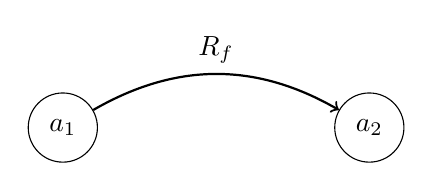
\begin{tikzpicture}[node distance=3cm]
					\node[state] (a) {$a_1$};
					\node[state, right=of a] (b) {$a_2$};
					\draw 
					(a) edge[->, thick, above, bend left] node{$R_f$} (b);
				\end{tikzpicture}
			\end{column}
			\begin{column}{0.5\textwidth}
				\centering
				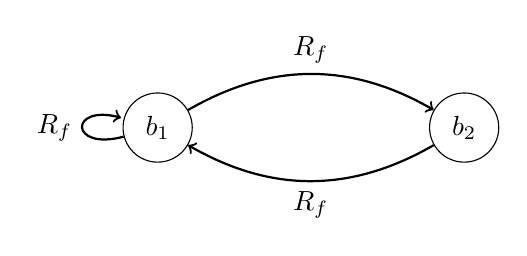
\begin{tikzpicture}[node distance=3cm]
					\node[state] (a) {$b_1$};
					\node[state, right=of a] (b) {$b_2$};
					\draw 
					(a) edge[->, thick, above, bend left] node{$R_f$} (b)
					(b) edge[->, thick, below, bend left] node{$R_f$} (a)
					(a) edge[->, thick, loop left] node{$R_f$} (a);
				\end{tikzpicture}
			\end{column}
		\end{columns}
	\end{frame}
	
	\begin{frame}{Non-Relational Acyclic Structures}
		\begin{itemize}
			\item Will define acyclicity w.r.t. the naive encoding
		\end{itemize}
		\begin{block}{Non-Relational Acyclic Structures}
			\begin{itemize}
				\item Let $\mathfrak A$ be a non-relational structure
				\item We call $\mathfrak A$ acyclic, if its naive encoding $\mathfrak A'$ is acyclic
			\end{itemize}
		\end{block}
	\end{frame}
	
	\begin{frame}{Total and Functional Structures as Encodings}
		\begin{itemize}
			\item Desired equivalence: 
			\begin{center}
				Non-relational, acyclic structure distinguishes $\mathfrak A$ and $\mathfrak B$ by homomorphism count \\ 
				? \\
				Naive RCR distinguishes $\mathfrak A$ and $\mathfrak B$
			\end{center}
			\item Result: Forward direction holds, backwards does not
			\item First step: Reformulate first statement:
			\begin{center}
				Some non-relational, acyclic structure dist. $\mathfrak A$ and $\mathfrak B$ by hom. count\\
				iff.\\
				Some total, functional and acyclic structure dist. encodings $\mathfrak A'$ and $\mathfrak B'$ by hom. count
			\end{center}
		\end{itemize}
	\end{frame}
	
	\begin{frame}{Enforcing Functionality}
		\begin{itemize}
			\item We can show:
			\begin{center}
				Acyclic $\sigma'$-structure dist. $\mathfrak A'$ and $\mathfrak B'$ by hom. count \\
				iff. \\
				Functional and acyclic $\sigma'$-structure dist. $\mathfrak A'$ and $\mathfrak B'$ by hom. count
			\end{center}
		\end{itemize}
		\emph{Proof idea:}
		\begin{itemize}
			\item Backwards direction is obvious
			\item Forwards direction eliminates collisions of the form $(\mathbf xy),(\mathbf xz)\in R_f$ by contracting $y$ and $z$
			\item This can be done while maintaining the homomorphisms and acyclicity and can be repeated until no collisions remain
		\end{itemize}
	\end{frame}
	
	\begin{frame}{Non-Enforceability of Totality}
		\begin{itemize}
			\item There are structures that are distinguished by naive RCR, but there is no acyclic and total structure that distinguishes the encodings by homomorphism count
			\item Define signature $\sigma=\{E/2,f/1\}$
			\item Two families of $\sigma$-structures $(\mathfrak A_i)_{i\in\mathbb N_{\geq 4}}$ and $(\mathfrak B_i)_{i\in\mathbb N_{\geq 4}}$
			\item For all $i\in \mathbb N_{\geq 4}$: Naive RCR distinguishes $\mathfrak A_i$ and $\mathfrak B_i$, but no acyclic and total structure can distinguish the encodings by hom. count
		\end{itemize}
	\end{frame}
	
	\begin{frame}{Structures that are distinguished by nRCR but not total structures i}
		\begin{columns}
			\begin{column}{0.25\textwidth}
				\centering
				\only<1->{
					\scalebox{0.8}{
						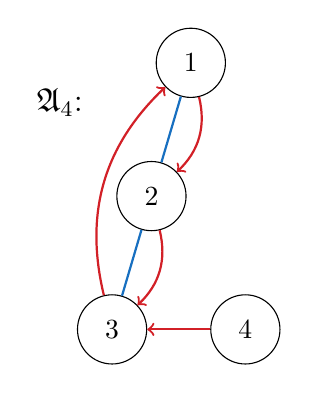
\begin{tikzpicture}[node distance=0.8cm]
							\node[state] (1) {$1$};
							\node[state, below =of 1, xshift=-0.5cm] (2) {$2$};
							\node[state, below =of 2, xshift=-0.5cm] (3) {$3$};
							\node[state, right =of 3] (4) {$4$};
							\node[left =of 1, yshift=-0.5cm] (label) {\large $\mathfrak A_4$:};
							\draw
							(1) edge[-, thick, rwth-blue] (2)
							(2) edge[-, thick, rwth-blue] (3)
							(1) edge[->, thick, bend left, rwth-red] (2)
							(2) edge[->, thick, bend left, rwth-red] (3)
							(3) edge[->, thick, bend left, rwth-red] (1)
							(4) edge[->, thick, rwth-red] (3);
						\end{tikzpicture}
					}
				}
			\end{column}
			
			\begin{column}{0.25\textwidth}
				\centering
				\only<1->{
					\scalebox{0.8}{
						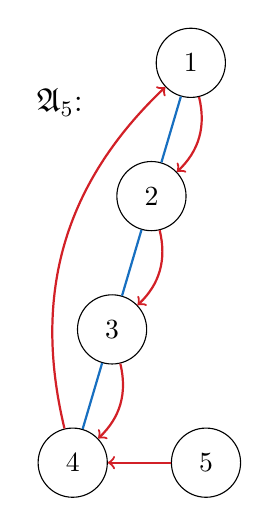
\begin{tikzpicture}[node distance=0.8cm]
							\node[state] (1) {$1$};
							\node[state, below =of 1, xshift=-0.5cm] (2) {$2$};
							\node[state, below =of 2, xshift=-0.5cm] (3) {$3$};
							\node[state, below =of 3, xshift=-0.5cm] (4) {$4$};
							\node[state, right =of 4] (5) {$5$};
							\node[left =of 1, yshift=-0.5cm] (label) {\large $\mathfrak A_5$:};
							\draw
							(1) edge[-, thick, rwth-blue] (2)
							(2) edge[-, thick, rwth-blue] (3)
							(3) edge[-, thick, rwth-blue] (4)
							(1) edge[->, thick, bend left, rwth-red] (2)
							(2) edge[->, thick, bend left, rwth-red] (3)
							(3) edge[->, thick, bend left, rwth-red] (4)
							(4) edge[->, thick, bend left, rwth-red] (1)
							(5) edge[->, thick, rwth-red] (4);
						\end{tikzpicture}
					}
				}
			\end{column}
			
			\begin{column}{0.25\textwidth}
				\centering
				\only<2>{
					\scalebox{0.8}{
						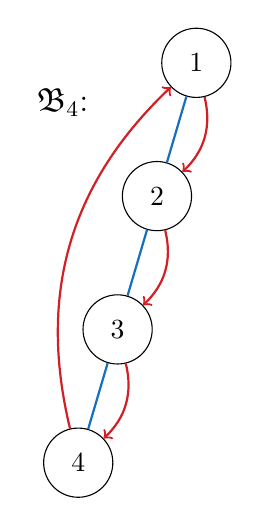
\begin{tikzpicture}[node distance=0.8cm]
							\node[state] (1) {$1$};
							\node[state, below =of 1, xshift=-0.5cm] (2) {$2$};
							\node[state, below =of 2, xshift=-0.5cm] (3) {$3$};
							\node[state, below =of 3, xshift=-0.5cm] (4) {$4$};
							\node[left =of 1, yshift=-0.5cm] (label) {\large $\mathfrak B_4$:};
							\draw
							(1) edge[-, thick, rwth-blue] (2)
							(2) edge[-, thick, rwth-blue] (3)
							(3) edge[-, thick, rwth-blue] (4)
							(1) edge[->, thick, bend left, rwth-red] (2)
							(2) edge[->, thick, bend left, rwth-red] (3)
							(3) edge[->, thick, bend left, rwth-red] (4)
							(4) edge[->, thick, bend left, rwth-red] (1);
						\end{tikzpicture}
					}
				}
			\end{column}
			
			
			
			\begin{column}{0.25\textwidth}
				\centering
				\only<2>{
					\scalebox{0.8}{
						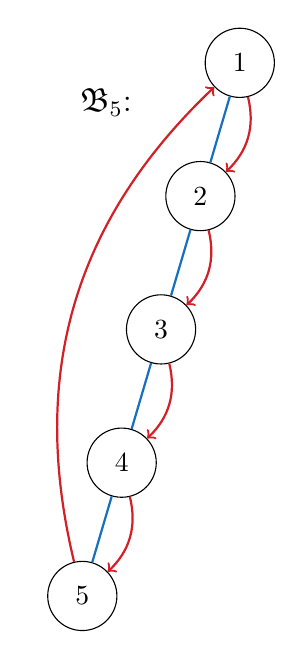
\begin{tikzpicture}[node distance=0.8cm]
							\node[state] (1) {$1$};
							\node[state, below =of 1, xshift=-0.5cm] (2) {$2$};
							\node[state, below =of 2, xshift=-0.5cm] (3) {$3$};
							\node[state, below =of 3, xshift=-0.5cm] (4) {$4$};
							\node[state, below =of 4, xshift=-0.5cm] (5) {$5$};
							\node[left =of 1, yshift=-0.5cm] (label) {\large $\mathfrak B_5$:};
							\draw
							(1) edge[-, thick, rwth-blue] (2)
							(2) edge[-, thick, rwth-blue] (3)
							(3) edge[-, thick, rwth-blue] (4)
							(4) edge[-, thick, rwth-blue] (5)
							(1) edge[->, thick, bend left, rwth-red] (2)
							(2) edge[->, thick, bend left, rwth-red] (3)
							(3) edge[->, thick, bend left, rwth-red] (4)
							(4) edge[->, thick, bend left, rwth-red] (5)
							(5) edge[->, thick, bend left, rwth-red] (1);
						\end{tikzpicture}
					}
				}
			\end{column}
		\end{columns}
	\end{frame}
	
	\begin{frame}{Structures that are distinguished by nRCR but not total structures ii}
		\begin{columns}
			\begin{column}{0.25\textwidth}
				\centering
				\scalebox{0.7}{
					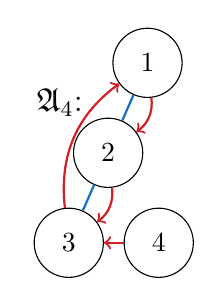
\begin{tikzpicture}[node distance=0.25cm]
						\node[state] (1) {$1$};
						\node[state, below =of 1, xshift=-0.5cm] (2) {$2$};
						\node[state, below =of 2, xshift=-0.5cm] (3) {$3$};
						\node[state, right =of 3] (4) {$4$};
						\node[left =of 1, yshift=-0.5cm] (label) {\large $\mathfrak A_4$:};
						\draw
						(1) edge[-, thick, rwth-blue] (2)
						(2) edge[-, thick, rwth-blue] (3)
						(1) edge[->, thick, bend left, rwth-red] (2)
						(2) edge[->, thick, bend left, rwth-red] (3)
						(3) edge[->, thick, bend left, rwth-red] (1)
						(4) edge[->, thick, rwth-red] (3);
					\end{tikzpicture}
				}
			\end{column}
			
			\begin{column}{0.25\textwidth}
				\centering
				\scalebox{0.7}{
					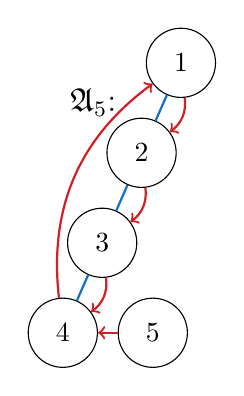
\begin{tikzpicture}[node distance=0.25cm]
						\node[state] (1) {$1$};
						\node[state, below =of 1, xshift=-0.5cm] (2) {$2$};
						\node[state, below =of 2, xshift=-0.5cm] (3) {$3$};
						\node[state, below =of 3, xshift=-0.5cm] (4) {$4$};
						\node[state, right =of 4] (5) {$5$};
						\node[left =of 1, yshift=-0.5cm] (label) {\large $\mathfrak A_5$:};
						\draw
						(1) edge[-, thick, rwth-blue] (2)
						(2) edge[-, thick, rwth-blue] (3)
						(3) edge[-, thick, rwth-blue] (4)
						(1) edge[->, thick, bend left, rwth-red] (2)
						(2) edge[->, thick, bend left, rwth-red] (3)
						(3) edge[->, thick, bend left, rwth-red] (4)
						(4) edge[->, thick, bend left, rwth-red] (1)
						(5) edge[->, thick, rwth-red] (4);
					\end{tikzpicture}
				}
			\end{column}
			
			\begin{column}{0.25\textwidth}
				\centering
				\scalebox{0.7}{
					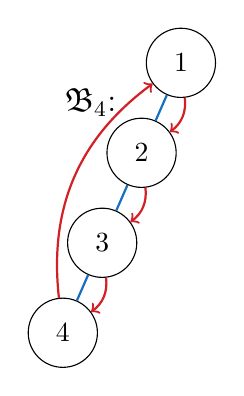
\begin{tikzpicture}[node distance=0.25cm]
						\node[state] (1) {$1$};
						\node[state, below =of 1, xshift=-0.5cm] (2) {$2$};
						\node[state, below =of 2, xshift=-0.5cm] (3) {$3$};
						\node[state, below =of 3, xshift=-0.5cm] (4) {$4$};
						\node[left =of 1, yshift=-0.5cm] (label) {\large $\mathfrak B_4$:};
						\draw
						(1) edge[-, thick, rwth-blue] (2)
						(2) edge[-, thick, rwth-blue] (3)
						(3) edge[-, thick, rwth-blue] (4)
						(1) edge[->, thick, bend left, rwth-red] (2)
						(2) edge[->, thick, bend left, rwth-red] (3)
						(3) edge[->, thick, bend left, rwth-red] (4)
						(4) edge[->, thick, bend left, rwth-red] (1);
					\end{tikzpicture}
				}
			\end{column}
			
			\begin{column}{0.25\textwidth}
				\centering
				\scalebox{0.7}{
					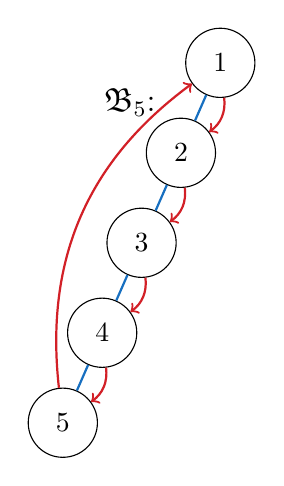
\begin{tikzpicture}[node distance=0.25cm]
						\node[state] (1) {$1$};
						\node[state, below =of 1, xshift=-0.5cm] (2) {$2$};
						\node[state, below =of 2, xshift=-0.5cm] (3) {$3$};
						\node[state, below =of 3, xshift=-0.5cm] (4) {$4$};
						\node[state, below =of 4, xshift=-0.5cm] (5) {$5$};
						\node[left =of 1, yshift=-0.5cm] (label) {\large $\mathfrak B_5$:};
						\draw
						(1) edge[-, thick, rwth-blue] (2)
						(2) edge[-, thick, rwth-blue] (3)
						(3) edge[-, thick, rwth-blue] (4)
						(4) edge[-, thick, rwth-blue] (5)
						(1) edge[->, thick, bend left, rwth-red] (2)
						(2) edge[->, thick, bend left, rwth-red] (3)
						(3) edge[->, thick, bend left, rwth-red] (4)
						(4) edge[->, thick, bend left, rwth-red] (5)
						(5) edge[->, thick, bend left, rwth-red] (1);
					\end{tikzpicture}
				}
			\end{column}
		\end{columns}
		\begin{itemize}
			\item Obviously distinguished by naive RCR
			\item If structure has $R_f$-loops or $R_f$-2-cycles, then no homomorphisms to either structure
			\item Because total, it has to contain larger $R_f$-cycles, but then cannot be acyclic
		\end{itemize}
	\end{frame}
	
	\begin{frame}{Results of combinatorial characterisation of naive RCR}
		We have the following results:
		\begin{center}
			Naive RCR distinguishes $\mathfrak A$ and $\mathfrak B$\\
			$\Updownarrow$\\
			There exists acyclic structure that dist. encodings $\mathfrak A'$ and $\mathfrak B'$ by hom. count\\
			$\Updownarrow$\\
			There exists acyclic and functional structure that dist. encodings by hom. count\\
			$\Uparrow$, but $\not\Downarrow$\\
			There exists acyclic, total and functional structure that dist. encodings by hom. count\\
			$\Updownarrow$\\
			There exists acyclic, non-relational structure that dist. $\mathfrak A$ and $\mathfrak B$ by hom. count
		\end{center}
	\end{frame}
	
	\section{RCR on Subclasses of Relational Structures}
	
	\begin{frame}{Restricting the Class of Structures}
		\begin{itemize}
			\item For what subclass $\mathcal S$ of relational structures do we have the following equivalence:
			\begin{center}
				Two structures from $\mathcal S$ get distinguished by RCR\\
				iff.\\
				There exists an acyclic structure from $\mathcal S$ that dist. the structures by hom. count
			\end{center}
			\item Does not hold for class of total structures
			\begin{itemize}
				\item[$\circ$] Encodings of classes of structures from before are total, but no total and acyclic structure dist. them by hom. count
			\end{itemize}
			\item Another class to investigate: Class of symmetric structures
		\end{itemize}
	\end{frame}
	
	\begin{frame}{Restriction to Symmetric Structures}
		\begin{itemize}
			\item Relational Structure is symmetric, if for every $k$-ary relation $R$ and for every $k$-tuple $\mathbf x\in R$, every permutation of the elements in $\mathbf x$ is also in $R$
			\pause
			\item For two symmetric structures we can show
			\begin{center}
				There exists acyclic structure dist. the structures by hom. count\\
				iff.\\
				There exists acyclic, symmetric structure dist. the structure by hom. count
			\end{center}
			\item From this, restriction to symmetric structures is possible
		\end{itemize}
	\end{frame}
	
	\section{Sketch of a Proof}
	
	\begin{frame}{Description of the Lemma}
		\begin{itemize}
			\item Lemma for translating $f^m(x_1)=x_2$ to a formula with a bounded number of applications of $f$ in series
			\item Used in proof of logical characterisation of RCR$_k$
		\end{itemize}
		\begin{block}{Lemma 4.6}
			A formula $\psi$ of the form $f^m(x_1)=x_2\in \GFC_1$ can be translated to a formula $\theta(x_1,x_2)\in\GFC_1$, such that:
			\begin{enumerate}
				\item They are equivalent for structures with $n$ elements
				\item There does not appear a term $f^i$ with $i>n$ in $\theta$
				\item $\theta$ is of the form $\bigvee \Phi$ and if $\theta$ is fulfilled, then there exists exactly one $\phi\in\Phi$ which is satisfied
			\end{enumerate}
		\end{block}
	\end{frame}
	
	\begin{frame}{Proof Idea}
		\begin{itemize}
			\item Elements $f^0(x),f^1(x),\dots,f^m(x)$ describe a path through a structure
			\item If $m>n$, there have to be $i,j\leq n$ such that $f^i(x)=f^j(x)$
			\item Path can be decomposed into:
			\begin{enumerate}
				\item Path to a cycle
				\item A cycle
				\item A last part of the cycle
			\end{enumerate}
			\item Define set $\mathcal I(n,m)$ as set of all such decomposition $(k,\ell,p)$
		\end{itemize}
		\centering
		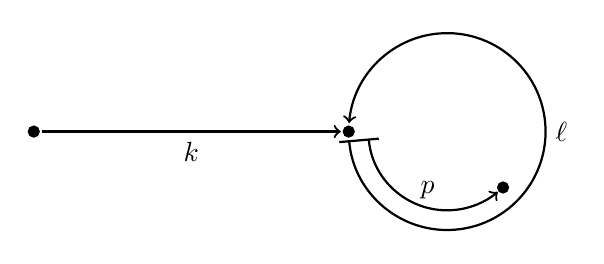
\begin{tikzpicture}
			\filldraw (-2, 0) circle (2pt); % Begin
			\draw[thick, ->] (-1.9, 0) -- node[below] {$k$} (1.9, 0) ;
			\filldraw (2, 0) circle (2pt); % End of k
			\draw[thick, |->] (3.25, 0) ++(-175:1.25) arc (-175:175:1.25);
			\node[xshift=4.7cm] {$\ell$};
			\draw[thick, |->] (3.25, 0) ++(-175:1) arc (-175:-50:1);
			\node[xshift=3cm, yshift=-0.75cm] {$p$};
			\filldraw (3.96, -0.71) circle (2pt);
		\end{tikzpicture}
	\end{frame}
	
	\begin{frame}[allowframebreaks]{Sketch of the Proof}
		\begin{itemize}
			\item Define $\theta(x_1,x_2)\coloneqq \bigvee_{(k,\ell,p)\in \mathcal I(n,m)} \zeta_{(k,\ell,p)}(x_1,x_2)$ where
			\begin{align*}
				\zeta_{(k,\ell,p)}(x_1,x_2)\coloneqq & f^{k+p}(x_1)=x_2 \land f^{k}(x_1)=f^{k+\ell}(x_1) \\
				& \land f^{k-1}(x_1)\neq f^{k-1+\ell}(x_1)  \\
				& \land \bigwedge_{0<\ell'<\ell}f^{k}(x_1)\neq f^{k+\ell'}(x_1)
			\end{align*}
			\begin{center}
				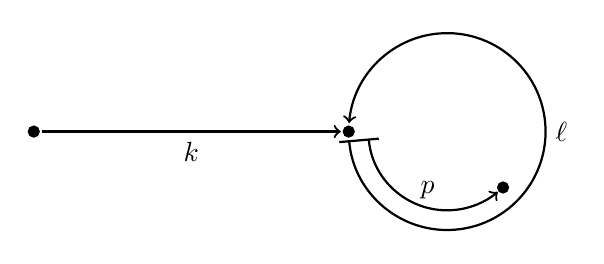
\begin{tikzpicture}
					\filldraw (-2, 0) circle (2pt); % Begin
					\draw[thick, ->] (-1.9, 0) -- node[below] {$k$} (1.9, 0) ;
					\filldraw (2, 0) circle (2pt); % End of k
					\draw[thick, |->] (3.25, 0) ++(-175:1.25) arc (-175:175:1.25);
					\node[xshift=4.7cm] {$\ell$};
					\draw[thick, |->] (3.25, 0) ++(-175:1) arc (-175:-50:1);
					\node[xshift=3cm, yshift=-0.75cm] {$p$};
					\filldraw (3.96, -0.71) circle (2pt);
				\end{tikzpicture}
			\end{center}
			\item $f^{k+p}(x_1)=x_2 \land f^{k}(x_1)=f^{k+\ell}(x_1)$ ensures that $(k,\ell,p)$ decomposes the path into a path to a cycle and the cycle itself
			\item $f^{k-1}(x_1)\neq f^{k-1+\ell}(x_1) \land \bigwedge_{0<\ell'<\ell}f^{k}(x_1)\neq f^{k+\ell'}(x_1)$ ensures that only the lexicographically smallest decomposition is satisfied
			\item[]
			\item If $\psi$ is satisfied, a smallest decomposition $(k,\ell,p)$ exists that decomposes the path of $f$
			\item Then it can be shown that $\zeta_{(k,\ell,p)}$ is satisfied, and because only the lexicographically smallest $(k,\ell,p)$ is satisfied, it is the only one
			\item[]
			\item If $\theta$ is satisfied, some $\zeta_{(k,\ell,p)}$ is satisfied
			\item This means that $(k,\ell,p)$ decomposes the path of $f$, therefore $\psi$ is also satisfied
		\end{itemize}
	\end{frame}
	
	\section{Conclusion}
	
	\begin{frame}{Conclusion}
		\begin{itemize}
			\item We presented classical CR and Scheidt's and Scheikardt's RCR algorithm
			\item We defined two possible ways to apply their algorithm to non-relational signatures
			\begin{itemize}
				\item Naive RCR
				\item RCR$_k$
			\end{itemize}
			\item We showed our results for the logical characterisations
			\begin{itemize}
				\item Naive RCR gets characterised by the nesting free fragment of counting logic
				\item RCR$_k$ gets characterised by the natural extension of $\GFC$ to non-relational signatures where terms have a maximal alternation depth of $k$
			\end{itemize}
			\item We disproved the characterisation by homomorphism counting
			\begin{itemize}
				\item Functionality can be enforced
				\item Totality cannot
			\end{itemize}
			\item We showed results for the restriction to two subclasses of the relational structures
			\begin{itemize}
				\item The restriction to total structures does not preserve the characterisation by hom. counting
				\item The restriction to symmetric structures does preserve it
			\end{itemize}
		\end{itemize}
	\end{frame}
	
	\appendix
	
	\begin{frame}{Equality between terms $t$ and alternations $\alpha$}
		\begin{itemize}
			\item For a term $t$ and a $\alpha\in\operatorname{Alters}^k_n(\sigma)$ we say $t=\alpha$, if:
			\item If $t=f^i(x)$, the $i$-times application of one function symbol $f$, and $\alpha=f^i$
			\item If $t=f^i(g^j(s(x)))$, where $f$ and $g$ are function symbols and $s$ is a term, and $\alpha=f^i\alpha'$ and $s=\alpha'$
			\item Informally, if $t$ is written using $\circ$, i.e. $f^i\circ g^j(x)$ instead of $f^i(g^j(x))$, the $\circ$ are omitted and then this equals $\alpha$
		\end{itemize}
	\end{frame}
	
\end{document}





















